\documentclass[a4paper,10pt]{article}
\usepackage[utf8]{inputenc}
\usepackage[english]{babel}
\usepackage[onehalfspacing]{setspace}
\usepackage{float}
\usepackage{biblatex}   % Using reference package
\addbibresource{mybibliography.bib}

\usepackage[nottoc]{tocbibind} %Adds "References" to the table of contents
\usepackage{graphicx}
\usepackage{hyperref}
%\graphicspath{/home/trung/Pictures/} \usepackage{float}
\hypersetup{
    colorlinks=true,
    linkcolor=blue,
    filecolor=magenta,      
    urlcolor=cyan,
}
%Document title, author and date (empty)
\title{Data Preprocessing}
\author{Trung Nguyen}
\date{}

%Beginning of the document
\begin{document}

\maketitle

\tableofcontents

\section{Introduction}

Machine learning “gives computers the ability to learn without being explicitly programmed” (Arthur Samuel, 1959).\newline
% When the technology is developed to a certain level, the users will not take much time to learn how to use it. The focus for the users will change from using tools for their work rather than learning the software behind.\newline
% We can start with an easy example of the modern smartphone, there are 3 main parties who involved: manufacturers, developer and the end users.
% Manufacturers: who are developed a smart phone 
% Developer: who developed an app.
% The end users: who use smart phone as a tools for their work and entertainment.

% In the applied data field are very similar (or ..), there are tools like Anaconda, Jupiter notebook, Online cloud platform.. etc.
% There are also a huge amount of libraries which have been developed by Scientist which use can take advantage on.
% The focus of this document will be put more on the end users.

There are five main tasks in the machine learning work flow.

\begin{itemize}
	\item Data collection and preparation.
	\item Feature selection and feature engineering.
	\item Choosing the machine learning algorithm (choosing the model) and training the model.
	\item Evaluating the model
	\item Model tweaking, parameter tuning and prediction.
\end{itemize}
Data Prepossessing is an important step. It transforms the raw data into an understandable format for the machine.The phrase “Garbage In ,Garbage Out” is particularly applicable to machine learning and data mining.

\begin{figure}[H]
	\centering
	
\includegraphics[width=0.8\columnwidth]{Pictures/GIGO.jpg}
	\caption[Short title]{GIGO}
	\label{fig:GIGO.}source:\cite{GIGO}
	\end{figure} 
If it is much irrelevant and redundant data or noisy and unreliable data then it is difficult to understand the pattern and our machine learning algorithm will not fit well to predict the correct estimations. (No Quality data, no correct predictions).  In the next chapter, the discussion on the basic step of preparing the data will be further discussed.

\begin{figure}[H]
	\centering
	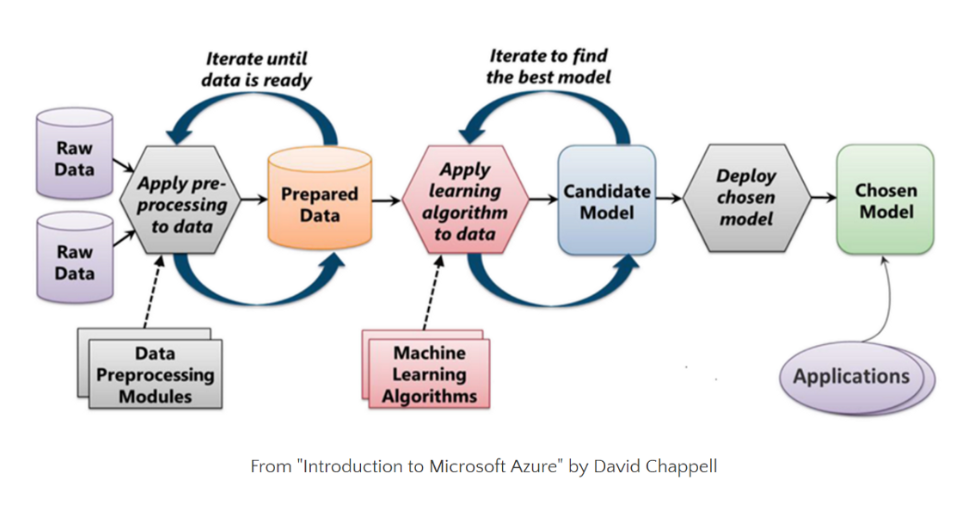
\includegraphics[width=0.8\columnwidth]{Pictures/ML_Cycles.png}
	\caption[Short title]{Machine Learning Process}
	\label{fig:ML.}source:\cite{David}
	\end{figure}

% ---------------------------------------------------------------------

\section{ Data Reprocessing and Data Visualization}

The visualization is not only important in the training steps but also important in the pre-processing steps.\newline
The raw data are often incomplete, noisy, and inconsistent. Visualizing the data help users understand more in-depth of the data sets.\newline
These are the most commonly used libraries in python.

\begin{itemize}
	\item \textbf{Numpy:} the fundamental package for computing and mathematical operations with Python.
	\item textbf{Pandas:} it is used for data manipulation and analysis.
	\item \textbf{Matplotlib :} python 2D plotting library.
	\item \textbf{Seaborn:} another python data visualization library based on matplotlib. It provides a high-level interface for drawing attractive and informative statistical graphics.
\end{itemize}

Try an notebook example of \href{https://www.kaggle.com/trungnguyen0987/data-pre-processing/edit/run/36863946}{data pre processing} here.

%----------------------------------------------------------------------

\section{Tips and Recommendation}

A cheat sheet is a concise set of notes used for quick reference (\href{https://en.wikipedia.org/wiki/Cheat_sheet}{wikipedia}).\newline
Looking into a cheat sheet will give a quick overview of the libraries function. An example of \href{https://s3.amazonaws.com/assets.datacamp.com/blog_assets/Numpy_Python_Cheat_Sheet.pdf}{Numpy cheat sheet } is showing below:

\begin{figure}[H]
	\centering
	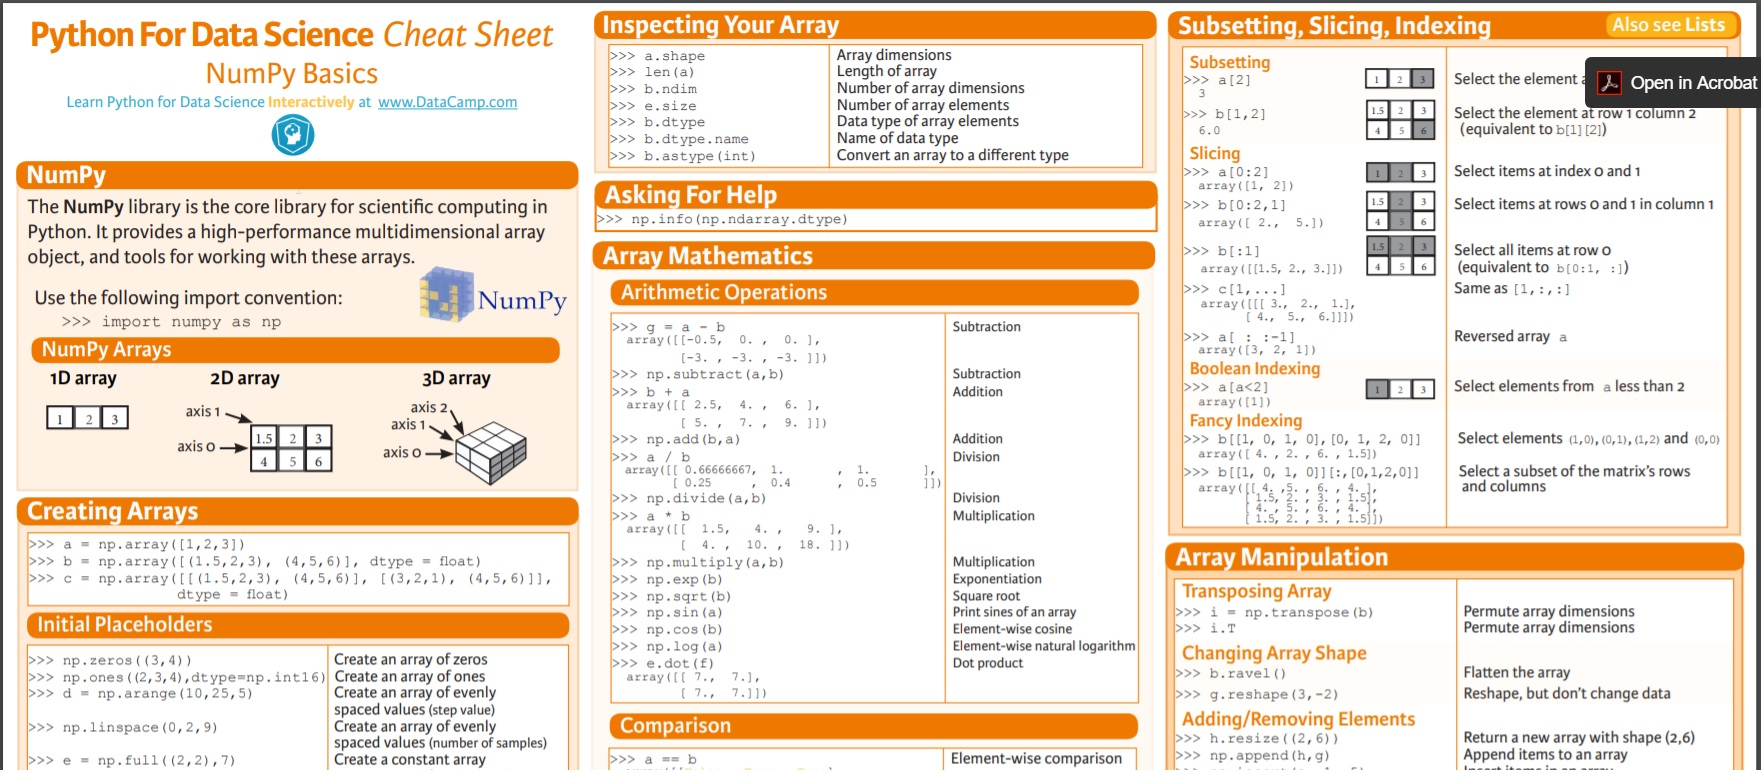
\includegraphics[width=0.8\columnwidth]{Pictures/numpy_cheatsheet.jpg}
	\caption[Short title]{Numpy cheat sheet}
	\label{fig:Numpy.}
	\end{figure}

Some useful cheat sheets for data manipulation:

\begin{itemize}
	\item \href{https://www.datacamp.com/community/blog/python-numpy-cheat-sheet}{Numpy basic cheat sheet}
	\item \href{https://www.datacamp.com/community/blog/python-pandas-cheat-sheet}{Panda basic cheat sheet}
	\item \href{https://www.datacamp.com/community/blog/pandas-cheat-sheet-python}{Pandas Data Wrangling Cheat Sheet}
	\item \href{https://www.datacamp.com/community/blog/python-matplotlib-cheat-sheet}{Matplotlib Cheat Sheet}
	\item \href{https://www.datacamp.com/community/blog/seaborn-cheat-sheet-python}{Seaborn Cheat Sheet}
	\item \href{https://s3.amazonaws.com/assets.datacamp.com/blog_assets/Python_Bokeh_Cheat_Sheet.pdf}{Bokeh Cheat Sheet}
\end{itemize}

There are a lot of tutorial from basic to advance with step to steps guideline which available from \href{https://medium.com/}{Medium} and \href{https://towardsdatascience.com/}{Towardsdatascience} blog spot. Read and try out those examples not only help to improve knowledge in the field but also get up to with the current development.



\medskip

% ---------------------------------------------------------------------

\section{Link to relevant information}

Some more example of data preprocessing on Medium and Kaggle notebook.\newline
\newline
Medium and towardsdatascience:

\begin{itemize}
	\item \href{https://medium.com/datadriveninvestor/data-p-reprocessing-a-significant-step-in-machine-learning-a749ce7e2d07}{Data Preprocessing- A significant step in Machine Learning}
	\item \href{https://towardsdatascience.com/data-preprocessing-concepts-fa946d11c825}{Data Preprocessing : Concepts}
	\item \href{https://towardsdatascience.com/data-pre-processing-techniques-you-should-know-8954662716d6}{Data Pre Processing Techniques You Should Know}
\end{itemize}. \newline

Kaggle Notebook:

\begin{itemize}
	\item \href{https://www.kaggle.com/gzuidhof/full-preprocessing-tutorial}{Full Preprocessing Tutorial Notebook}

\end{itemize}

%-------------------------------------------------------------------------

\section{List of Documentation}

\begin{enumerate}
  \item Python Guideline for Beginner.
  \item Setting up Online Python Notebook
  \item Data Preprocessing
  \item update...
\end{enumerate}

\vspace{1cm}
\vspace{1cm}




%----------------------------------------------------------------

\section{Recommendation Courses}

\href{https://www.coursera.org/learn/machine-learning}{Machine learning by Andrew Ng.}\\
\href{https://www.usfca.edu/data-institute/certificates/deep-learning-part-one}{Deep Learning using FastAI  by Jeremy Howard.}


%----------------------------------------------------------------


%Bibliographic references
\printbibliography

\end{document}
